\documentclass[12pt, a4paper, fleqn, titlepage]{article}

%Packages to use
\usepackage[utf8]{inputenc}
\usepackage{enumerate}
\usepackage{hyperref}
\usepackage{setspace}
\usepackage{ragged2e}
\usepackage{algorithm2e}
\usepackage{graphicx}
\graphicspath{ ./ }


\title{Introduction to Parallel and Distributed Computing Lab 1}
\author{Kweku Andoh Yamoah(71712022)}
\date{\today}

%Starting assignment
\doublespacing

\begin{document}
\maketitle
\justify
%Part one of Lab
\section{Top HPC Machines in the World(First 5)}
    \subsection{Super Computer FUGAKU}
        \begin{flushleft}
            \begin{enumerate}[\textbullet]
                \item \textbf{Rank}: 1
                \item \textbf{Location:} 
                    Located at the RIKEN Centre for Computational Science in Kobe, Japan
                \item \textbf{URL:} 
                    \url{https://www.r-ccs.riken.jp/en/fugaku/project}
                \item \textbf{Manufacturer:} Manufactured by Fujitsu
                \item \textbf{Memory:} 5,087,232 GB
                \item \textbf{Number of Cores:} 7,630,848
                \item \textbf{Processor Type:} A64FX 48C 2.2GHz
                \item \textbf{Interconnect:} Tofu interconnect D
                \item \textbf{Linpack Performance:} 442,010 TFlop/s
                \item \textbf{Theoretical Peak:} 537,212 TFlop/s
                \item \textbf{Power Consumption:} 29,899.23 kW (Optimized: 26248.36 kW)
                \item \textbf{Operating System:} Red Hat Enterprise Linux
                \item \textbf{Any Other Interesting Features:}
                    \begin{enumerate}
                        \item Compiler: FUJITSU Software Technical Computing Suite V4.0
                        \item Math Library: FUJITSU Software Technical Computing Suite V4.0
                        \item MPI: FUJITSU Software Technical Computing Suite V4.0
                    \end{enumerate}
            \end{enumerate}
        \end{flushleft}

    \subsection{SUMMIT}
        \begin{flushleft}
            \begin{enumerate}[\textbullet]
                \item \textbf{Rank}: 2
                \item \textbf{Location:} 
                    Located at the DOE/SC/Oak Ridge National Laboratory in Oak Ridge, USA
                \item \textbf{URL:} 
                    \url{http://www.olcf.ornl.gov/olcf-resources/compute-systems/summit/}
                \item \textbf{Manufacturer:} Manufactured by IBM
                \item \textbf{Memory:} 2,801,664 GB
                \item \textbf{Number of Cores:} 2,414,592
                \item \textbf{Processor Type:} IBM POWER9 22C 3.07GHz
                \item \textbf{Interconnect:} Dual-rail Mellanox EDR Infiniband
                \item \textbf{Linpack Performance:} 148,600 TFlop/s
                \item \textbf{Theoretical Peak:} 200,795 TFlop/s
                \item \textbf{Power Consumption:} 10,096.00 kW (Submitted)
                \item \textbf{Operating System:} RHEL 7.4
                \item \textbf{Any Other Interesting Features:}
                    \begin{enumerate}
                        \item Compiler: XLC, nvcc
                        \item Math Library: ESSL, CUBLAS 9.2
                        \item MPI: Spectrum MPI
                    \end{enumerate}
            \end{enumerate}
        \end{flushleft}
    
    
    \subsection{SIERRA}
        \begin{flushleft}
            \begin{enumerate}[\textbullet]
                \item \textbf{Rank}: 3
                \item \textbf{Location:} 
                    Located at the DOE/NNSA/LLNL in Livermore, USA
                \item \textbf{URL:} 
                    \url{https://hpc.llnl.gov/hardware/platforms/sierra}
                \item \textbf{Manufacturer:} Manufactured by IBM / NVIDIA / Mellanox
                \item \textbf{Memory:} 1,382,400 GB
                \item \textbf{Number of Cores:} 1,572,480
                \item \textbf{Processor Type:} IBM POWER9 22C 3.1GHz
                \item \textbf{Interconnect:} Dual-rail Mellanox EDR Infiniband
                \item \textbf{Linpack Performance:} 94,640 TFlop/s
                \item \textbf{Theoretical Peak:} 125,712 TFlop/s
                \item \textbf{Power Consumption:} 7,438.28 kW (Submitted)
                \item \textbf{Operating System:} Red Hat Enterprise Linux
                \item \textbf{Any Other Interesting Features:}
                    \begin{enumerate}
                        \item Compiler: IBM XLC
                        \item Math Library: ESSL, CUBLAS 9.2
                        \item MPI: IBM Spectrum MPI
                    \end{enumerate}
            \end{enumerate}
        \end{flushleft}

    \subsection{SUNWAY TAIHULIGHT}
        \begin{flushleft}
            \begin{enumerate}[\textbullet]
                \item \textbf{Rank}: 4
                \item \textbf{Location:} 
                    Located at the National Supercomputing Center in Wuxi, China
                \item \textbf{URL:} 
                    \url{Not Available}
                \item \textbf{Manufacturer:} Manufactured by NRCPC
                \item \textbf{Memory:} 1,310,720 GB
                \item \textbf{Number of Cores:} 10,649,600
                \item \textbf{Processor Type:} Sunway SW26010 260C 1.45GHz
                \item \textbf{Interconnect:} Sunway
                \item \textbf{Linpack Performance:} 93,014.6 TFlop/s
                \item \textbf{Theoretical Peak:} 125,436  TFlop/s
                \item \textbf{Power Consumption:} 15,371.00 kW (Submitted)
                \item \textbf{Operating System:} Sunway RaiseOS 2.0.5
                \item \textbf{Any Other Interesting Features:}
                    \begin{enumerate}
                        \item Compiler: Not Available
                        \item Math Library: Not Available
                        \item MPI: Not Available
                    \end{enumerate}
            \end{enumerate}
        \end{flushleft}

    \subsection{SELENE}
        \begin{flushleft}
            \begin{enumerate}[\textbullet]
                \item \textbf{Rank}: 4
                \item \textbf{Location:} 
                    Located at the National Supercomputing Center in Wuxi, China
                \item \textbf{URL:} 
                    \url{https://www.nvidia.com/DGXSuperPOD}
                \item \textbf{Manufacturer:} Manufactured by Nvidia
                \item \textbf{Memory:} 1,120,000 GB
                \item \textbf{Number of Cores:} 555,520
                \item \textbf{Processor Type:} AMD EPYC 7742 64C 2.25GHz
                \item \textbf{Interconnect:} Mellanox HDR Infiniband
                \item \textbf{Linpack Performance:} 63,460 TFlop/s
                \item \textbf{Theoretical Peak:} 79,215  TFlop/s
                \item \textbf{Power Consumption:} 2,646.00  kW (Submitted)
                \item \textbf{Operating System:} Ubuntu 20.04.1 LTS
                \item \textbf{Any Other Interesting Features:}
                    \begin{enumerate}
                        \item Compiler: NVIDIA NVCC V11, Intel Composer 2020.0.166
                        \item Math Library: NVIDIA CUDA V11.0.148, Intel MKL 2020.0.166
                        \item MPI: OpenMPI 4.0.3
                    \end{enumerate}
            \end{enumerate}
        \end{flushleft}


\section{Top HPC Machine Africa}
    \subsection{LENGAU}
        \begin{flushleft}
            \begin{enumerate}[\textbullet]
                \item \textbf{Rank}: 4
                \item \textbf{Location:} 
                    Located at the Centre for High Performance Computing in Cape Town, South Africa
                \item \textbf{URL:} 
                    \url{http://www.chpc.ac.za/}
                \item \textbf{Manufacturer:} Manufactured by Dell EMC
                \item \textbf{Memory:} 175,232 GB
                \item \textbf{Number of Cores:} 32,856
                \item \textbf{Processor Type:} Xeon E5-2690v3 12C 2.6GHz
                \item \textbf{Interconnect:} Infiniband FDR
                \item \textbf{Linpack Performance:} 1,029.32  TFlop/s
                \item \textbf{Theoretical Peak:} 1,366.81  TFlop/s
                \item \textbf{Power Consumption:} 685.00  kW (Submitted)
                \item \textbf{Operating System:} CentOS
                \item \textbf{Any Other Interesting Features:}
                    \begin{enumerate}
                        \item Compiler: Not Available
                        \item Math Library: Intel MKL
                        \item MPI: Intel MPI
                    \end{enumerate}
            \end{enumerate}
        \end{flushleft}
\section{Applications of HPC machines in Ghana}
    
        In the context of using HPC machines in Ghana, I will focus on Weather forecasting, Oil and gas exploration and Research. 
        \subsection{HPC in Weather Forecasting}
        Weather predicting depends on data and various input parameters. The can be obtained from weather stations and satellite images(only if we have some as a country). This data can be stored and fed to an HPC machine. The machine comes with hardware and software that enables the processing, analysis and visualising of data. When this is done, the country will be able to numerically and empirically predict the changes in weather pattern way ahead of time. This will go a long to inform the Ministry of Agriculture on the policies they should implement for any given season since the nation depends heavily on the exportation of cash crops. Also, HPC systems will give the nation the chance to prepare adequately for any incoming natural disaster since it will be well known before hand. This helps save money spent on recovery after the event of a natural disaster.

        \subsection{HPC in Oil and Gas Exploration}
        Ghana discovered its first oil fields in 2007 called Jubilee Field. To become a global exporter and help meet the global demand for crude, the nation needs to keep searching for new sources of crude along the Gulf of Guinea. The solution to this problem lies in the utilisation HPC machines in the exploration across the gulf. Because with usage of HPC machines, the country can reduce the time it takes to analyse exploratory data from weeks to months. For example, the world's fastest commercial HPC is able to simulate 15 years' worth of oil reservoir production in just 28 minutes(cite). What great potential that is available for Ghana to generate more revenue.

        \subsection{HPC in Research}
        The final area that HPC can have vast impact is on the sort of Research publications academia pushes from the country. An HPC machine acquired for the purposes of fostering research in the country will help ensure that the nation produces research papers that are revolutionary and have vast industrial applications. It will also spark interest in parallel and distributed computing across the country.

    

\section{Challenges of operating HPC machines in Ghana}
    
        The first challenge that can limit the operation of an HPC machine in Ghana is energy consumption. Some HPC systems consume much electricity like what will be consumed by a typical settlement. This can make ECG not want to supply electricity for the operation of the HPC machine.Also, HPC machines generate so much heat that they have to be cooled down and this requires electrical energy consumption.\\
        The second challenge, is the location of the HPC. If an HPC machine is going to be purchased for the country, then an ideal situation site becomes a challenge. Because, where the HPC machine will be located must make it relatively accessible to all potential users. Also, the location becomes necessary because of energy and cooling needs.\\
        Finally, the last issue on the horizon is the maintenance of the machine. Ghanaians have a history of bad maintenance culture. So, the acquisition of the machine should come with the requirement that experts are available at the site of deployment to ensure the continuos use of the system.
    

\section{Part Two}
    \begin{enumerate}[a.]
        \item I chose to dual boot my Linux programing environment with Ubuntu 20.04 LTS running with Windows 10.
        \item My preferred editor was visual studio code because it was easier to transfer my settings and extensions from Windows to Linux.
        \item I played around with the python interpreter in Linux. I wrote a simple program \emph{sample.py}. To run the program, I navigated to working directory and a run the command \emph{python3 sample.py}. This is how the command looks in terminal:
    \end{enumerate}

    \begin{center}
        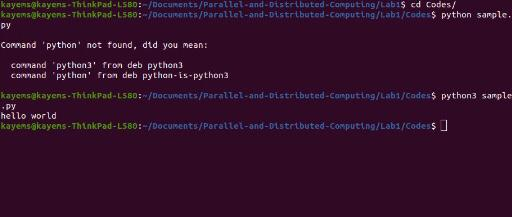
\includegraphics[width= 20cm,height = 5cm, keepaspectratio,scale=0.8]{py}
    \end{center}
        
    \begin{enumerate}[d.]
        \item Next I wrote a program that utilises the PThread library. The goal of the program was to print the thread numbers and the return value of the threads. This is how the compilation and results turned out: 
    \end{enumerate}

    \begin{center}
        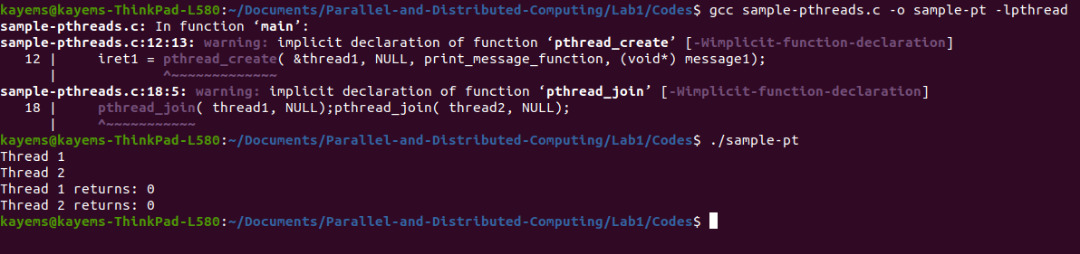
\includegraphics[width= 17cm,height = 8cm, keepaspectratio,scale=0.5]{pt}
    \end{center}

    \begin{enumerate}[e.]
        \item Finally, I used the gcc compiler to compile a program that utilises the OpenMP library in a Unix environment. The name of the files was \emph{sample-omp.c}. This was the results I obtained in the terminal:
        
    \end{enumerate}

    \begin{center}
        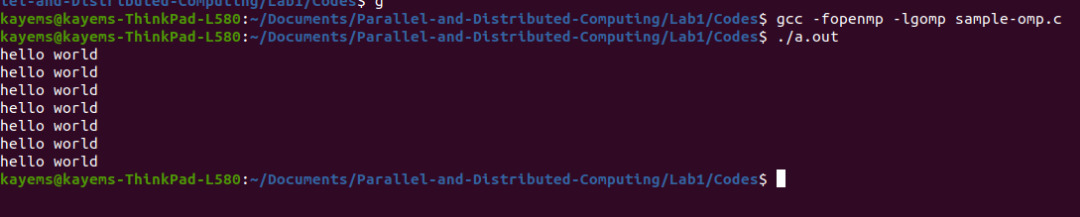
\includegraphics[width= 17cm,height = 8cm, keepaspectratio,scale=0.5]{omp}
    \end{center}
\end{document}